\section{Introduction}
\begin{itemize}
    \item If we remove the constraint on the number of physical processors we have available to us, and if all processors could communicate with minimal, predictable latency, \emph{how would we design distributed applications?}
    \item We believe that many applications have inherent parallelizability that cannot be harnessed today because of large, unpredictable network latencies provided by today's communication infrastructure.
    \item If we eliminate these issues then we believe that we would re-implement distributed applications at a much finer granularity to harness as much parallelism as possible.
    \item To understand the importance of minimizing both average and tail latency, let's consider a simple example application. This application consists of $N$ potentially parallelizable tasks that can either be executed locally or on a remote core via an RPC. The job is considered completed once all tasks have been executed. Let's assume that executing the task locally requires $x$ us, whereas executing the task via RPC requires $(r)x$ us for some $r>=1$. We will also make the simplifying assumption that we have an ideal network with infinite capacity (i.e. negligible RPC serialization delay). Let $K$ be the number of RPCs that are issued (i.e. the number of remote cores that are utilized). The point at which sending out additional RPCs is no longer beneficial is when the total job completion time is defined by the following equation: $(N - K)x = (r)x$. This is the point when the tasks that are executed locally complete at the exact same time as all the issued RPCs. Solving this equation for $K$ yields: $K = N - r$. If we were to send out an additional RPC then the local core would be sitting idle while it waits for the RPCs to complete and hence total job completion time will not decrease. So if $r = 10$ (i.e. RPCs take 10 times as long as local execution) then we would want to send out $N-10$ RPCs and execute 10 tasks locally. Whereas, if $r = 1$ then we would issue RPCs for all but one task, resulting in a 10x reduction in total job completion time.
    \item From this simple example, we can clearly see that reducing RPC completion time allows us to utilize more cores and achieve significant performance gains for applications.
    \item However, the above simple model assumed that RPC completion times were deterministic. In reality, RPC completion times are characterized by a probability distribution. In this case, the total job completion time is given by: $(N - K)x =$ max of $K$ samples drawn from RPC completion time distribution. This means that in order to improve performance we need to reduce the tail of the distribution. This observation is not new and has been the motivation for much recent work~\cite{shinjuku, shenango, rpcvalet}.
    \item Figure~\ref{fig:nanoservice-sim} shows what we aim to achieve. We aim to reduce both the average and the standard deviation of the RPC completion time distribution by an order of magnitude in order to reduce total application runtime by utilizing as many cores as possible.
    \item The NanoPU is the first attempt to realize this vision.
    \begin{itemize}
        \item Explicitly designed to scale out. In order to harness as much parallelism as possible we need to think beyond a single chip and build an architecture that is highly optimized for compute intensive networking applications in order to scale out.
        \item Goal is to put as many cores into the network as possible. We want to put \emph{cores} into the network without letting memory get in the way. \chang{I think we should justify the memory bypassing design.}
        \item Goal is to minimize \emph{both} average and tail latency to provide both optimal and predictable performance.
        \item Goal is to minimize the overhead 
    \end{itemize}
    \item The nanoservices framework is a new way of building distributed applications that is very different from how distributed applications are designed today.
    \item We believe that many applications can be re-implemented using the nanoservices framework:
    \begin{itemize}
        \item Physical simulations
        \item Neural Network Inference and Training (or matrix operations more generally)
        \item Graphics processing
        \item State space search algorithms
    \end{itemize}
    \item Today's best practices for designing distributed applications encourage developers to hide network latency as much as possible by overlapping communication with computation. Developers are forced to batch what would be many small messages into fewer large messages in order to amortize high communication overheads. This approach prevents modern implementations from harnessing all of the parallelism in distributed applications, thus sacrificing performance.
    \item In order to overcome this significant problem we propose the NanoPU which minimizes: (1) the tail RPC completion time by introducing NIC driven thread scheduling, (2) the average RPC completion time by implementing a fast path to the heart of the CPU, and (3) minimizes communication overhead by implementing NIC-terminated transport protocol.
\end{itemize}

\begin{figure}
  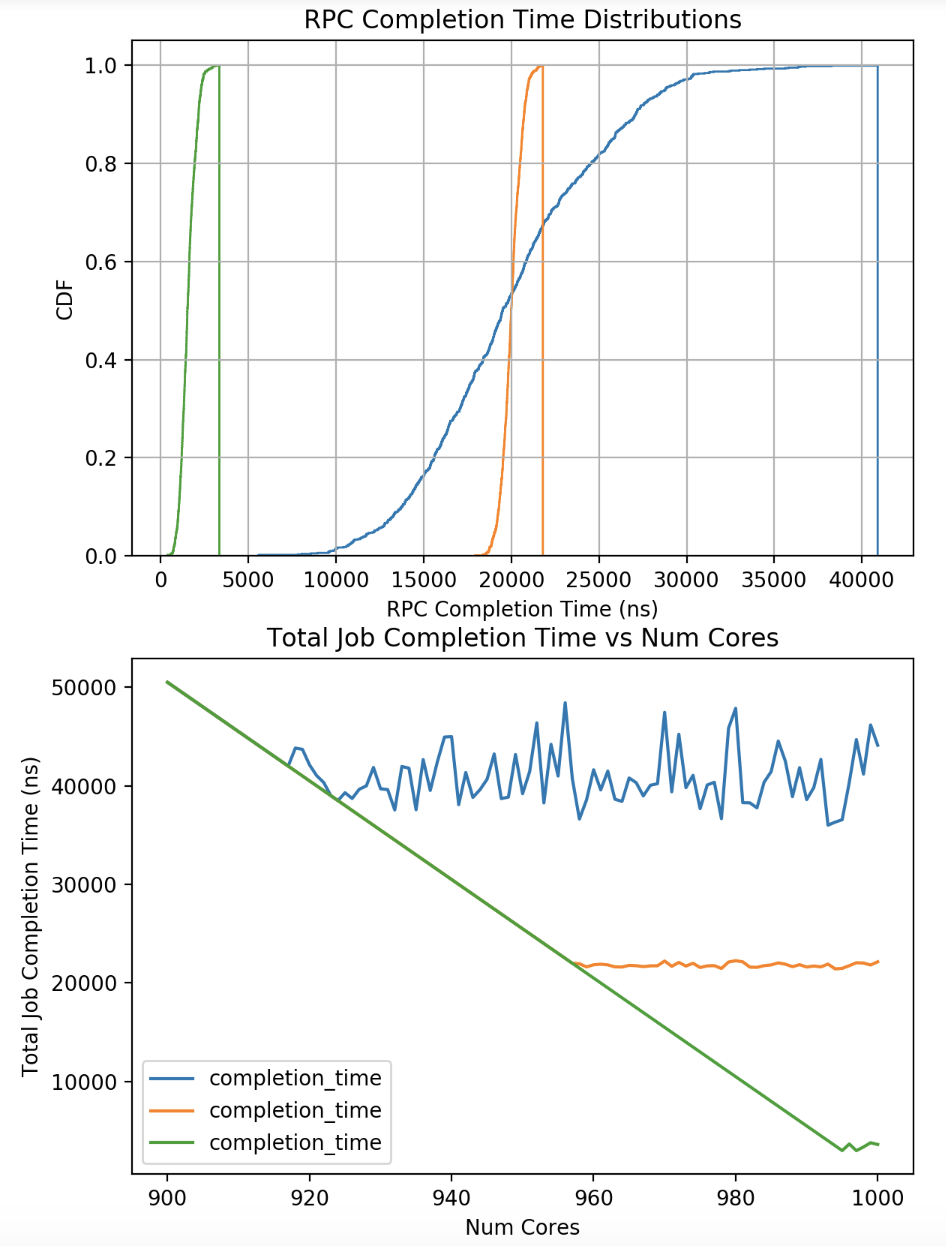
\includegraphics[width=\linewidth]{./figures/nanoservice-sim}
  \caption{RPC completion time distributions and their corresponding impact on total application runtime for a simple example application.}
  \label{fig:nanoservice-sim}
\end{figure}